\documentclass[a4paper]{article} % A4 paper and 11pt font size


\usepackage{tikz}
\usepackage{tikz-feynman}


%%%%%%%%%%%%%%%CATE'S PREAMBLE BIT%%%%%%%%%%%%%%%%

\usepackage{tikz}
\usetikzlibrary{arrows,shapes}
\usetikzlibrary{trees}
\usetikzlibrary{patterns}
\usetikzlibrary{matrix,arrows} 				% For commutative diagram
											% http://www.felixl.de/commu.pdf
\usetikzlibrary{positioning}				% For "above of=" commands
\usetikzlibrary{calc,through}				% For coordinates
\usetikzlibrary{decorations.pathreplacing}  % For curly braces
% http://www.math.ucla.edu/~getreuer/tikz.html
\usepackage{pgffor}							% For repeating patterns

\usetikzlibrary{decorations.pathmorphing}	% For Feynman Diagrams
\usetikzlibrary{decorations.markings}
\tikzset{
	% >=stealth', %%  Uncomment for more conventional arrows
    vector/.style={decorate, decoration={snake}, draw},
	provector/.style={decorate, decoration={snake,amplitude=2.5pt}, draw},
	antivector/.style={decorate, decoration={snake,amplitude=-2.5pt}, draw},
    fermion/.style={draw=black, postaction={decorate},
        decoration={markings,mark=at position .55 with {\arrow[draw=black]{>}}}},
    fermionbar/.style={draw=black, postaction={decorate},
        decoration={markings,mark=at position .55 with {\arrow[draw=black]{<}}}},
    fermionnoarrow/.style={draw=black},
    gluon/.style={decorate, draw=black,
        decoration={coil,amplitude=4pt, segment length=5pt}},
    scalar/.style={dashed,draw=black, postaction={decorate},
        decoration={markings,mark=at position .55 with {\arrow[draw=black]{>}}}},
    scalarbar/.style={dashed,draw=black, postaction={decorate},
        decoration={markings,mark=at position .55 with {\arrow[draw=black]{<}}}},
    scalarnoarrow/.style={dashed,draw=black},
    electron/.style={draw=black, postaction={decorate},
        decoration={markings,mark=at position .55 with {\arrow[draw=black]{>}}}},
    bigvector/.style={decorate, decoration={snake,amplitude=4pt}, draw},
    arrow/.style={draw=black, postaction={decorate},
        decoration={markings,mark=at position 1 with {\arrow[draw=black]{>}}}},
}

% TIKZ - for block diagrams, 
% from http://www.texample.net/tikz/examples/control-system-principles/
% \usetikzlibrary{shapes,arrows}
\tikzstyle{block} = [draw, rectangle, 
    minimum height=3em, minimum width=6earticlem]

%%%%%%%%%%%%%%END CATE'S PREAMBLE BIT%%%%%%%%%%%%%

\tikzset{>=latex}


\begin{document}
\pagestyle{empty}

%--------- tau -> pi nu
\begin{figure}[h]
\centering
{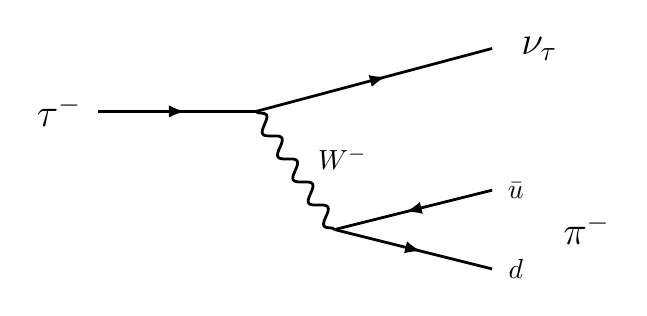
\begin{tikzpicture}[line width=1 pt]
\draw [fermion] (1,3)--(3,3);
\node at (0.5,3) {{\Large $\tau^{-}$}};


\draw [fermion] (3,3)--(6,3.8);
\node at (6.6,3.8) {{\Large $\nu_{\tau}$}};

\draw [vector] (3,3)--(4,1.5);
\node at (4.1,2.4) {$W^-$};

\draw [fermionbar] (4,1.5)--(6,2);
\draw [fermion] (4,1.5)--(6,1);
\node at (6.3,2) {$\bar{u}$};
\node at (6.3,1) {$d$};
\node at (7.2,1.5) {\Large{$\pi^-$}};
\end{tikzpicture}}
\end{figure}


%--------- tau -> mu nu nu
\begin{figure}[h]
\centering
{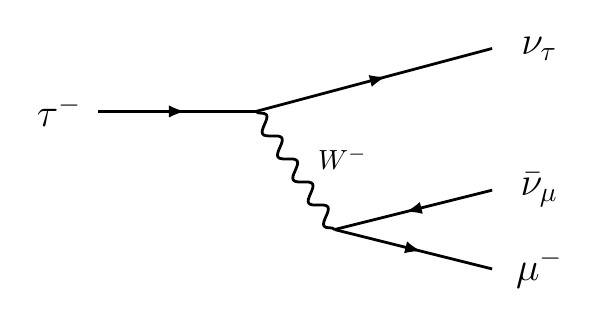
\begin{tikzpicture}[line width=1 pt]
\draw [fermion] (1,3)--(3,3);
\node at (0.5,3) {{\Large $\tau^{-}$}};


\draw [fermion] (3,3)--(6,3.8);
\node at (6.6,3.8) {{\Large $\nu_{\tau}$}};

\draw [vector] (3,3)--(4,1.5);
\node at (4.1,2.4) {$W^-$};

\draw [fermionbar] (4,1.5)--(6,2);
\draw [fermion] (4,1.5)--(6,1);
\node at (6.6,2) {{\Large $\bar{\nu}_{\mu}$}};
\node at (6.6,1) {{\Large $\mu^{-}$}};
\end{tikzpicture}}
\end{figure}

%--------- e e -> mu mu gamma
\begin{figure}[h]
\centering
{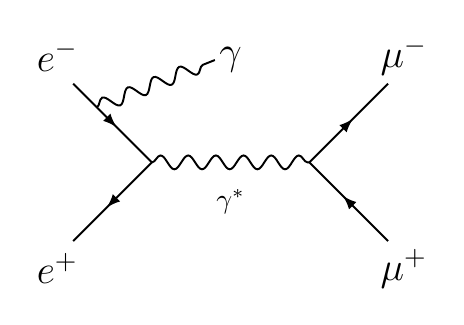
\begin{tikzpicture}[line width=0.7 pt]
%LEFT SIDE
\draw [fermion] (0,4)--(1,3);
	\node at (-0.2,4.35) {{\Large $e^-$}};
\draw [fermionbar] (0,2)--(1,3);
	\node at (-0.2,1.65) {{\Large $e^+$}};
\draw [vector] (0.3,3.7)--(1.8,4.3);
	\node at (2,4.3) {{\Large $\gamma$}};

%PROPAGATOR
\draw [vector] (1,3)--(3,3);
	\node at (2,2.5) {$\gamma^{\ast}$};

%RIGHT SIDE
\draw [fermion] (3,3)--(4,4);
	\node at (4.2,4.35) {{\Large $\mu^{-}$}};
\draw [fermionbar] (3,3)--(4,2);
	\node at (4.2,1.65) {{\Large $\mu^{+}$}};
\end{tikzpicture}}
\end{figure}




\end{document}







